%%%%%%%%%%%%%%%%%%%%%%%%%%%%%%%%%%%%%%%%%%%%%%%%%%%%%%%%%%%%%%%%%%%%%%
\clearpage
\section{Building HOPSPACK}
\label{sec:build}

HOPSPACK is written with the intent of allowing user modifications and
extensions.  All code is written in C++.  HOPSPACK uses the CMake build
system (\href{http://cmake.org/}{http://cmake.org/}) to support compilation on
multiple platforms, including Linux, Windows, and Mac OSX.  This section
describes the process of installing source code, third party libraries,
and building HOPSPACK executables.
\SECREF{sec:extend} provides examples of modifying or extending
the source code.

Several steps are required to build HOPSPACK.  A quick outline is below,
and full details for various platforms follow.
\begin{list}{x}{\setlength{\itemindent}{20pt}
                \setlength{\itemsep}{-4pt}
                \setlength{\labelsep}{10pt}}
  \item[\ref{subinstall:DN}] Download and unpack HOPSPACK source code.
  \item[\ref{subinstall:CM}] Download and install CMake toolset.
  \item[\ref{subinstall:LA}] Obtain or build an LAPACK library (if linear
                             constraints are used).
  \item[\ref{subinstall:SR}] Build and test a ``serial'' (single processor)
                             HOPSPACK executable.
  \item[\ref{subinstall:MT}] Build and test an ``mt'' (multithreaded)
                             HOPSPACK executable.
  \item[\ref{subinstall:MP}] Build and test an ``mpi'' (multiprocessor)
                             HOPSPACK executable.
  \item[\ref{subinstall:ED}] Complete list of build options.
\end{list}


%%%%%%%%%%%%%%%%%%%%
\subsection{Download HOPSPACK Source Code}
\label{subinstall:DN}

Follow the links at
\vspace{-11pt}
\begin{tabbing}
  xxx \= xxxxxxxxx \= \kill
  \> \href{https://software.sandia.gov/trac/hopspack}
          {https://software.sandia.gov/trac/hopspack}
\end{tabbing}
\vspace{-11pt}
to find the download page.  Please register your email address with
accurate and complete information.  We ask for this information as a
courtesy in exchange for our free software.  Having accurate user data allows
us to better ascertain in what way HOPSPACK is used, which may influence
future development.  Your email address will remain strictly confidential
and will not be used unless you request to be on the HOPSPACK Users Mailing List.
Remember the email address you register so you can registration the next time.

Download the source code.  For convenience, it is supplied in both Windows
compressed file form and Unix compressed tar file form.  The contents are
the same.

Save the compressed file to any directory and unzip it.
You should see a directory structure like the following:
\vspace{-11pt}
\begin{tabbing}
  xxxxxxxxx \= xxx \= xxx \= xxxxxxxxxxxxxxxxxx \= \kill
  \> {\sf hopspack-\HOPSVER.x-src}  \\
  \> \> {\sf doc}                   \\
  \> \> {\sf examples}              \\
  \> \> {\sf src}                   \\
  \> \> {\sf test}
\end{tabbing}


%%%%%%%%%%%%%%%%%%%%
\subsection{Download and Install CMake}
\label{subinstall:CM}

CMake is a leading open-source build system that supports multiple operating
systems.  You need to download a CMake binary distribution
(typically, 5-10 Mbytes in size) appropriate for your operating system
and install it.  If HOPSPACK will run on different machines, then install
CMake on each target machine.
The installation creates a CMake tool that will be used to construct
platform-specific build scripts for compiling HOPSPACK source code.

Visit \href{http://cmake.org/}{http://cmake.org/} and find a recent release
of CMake for your target operating system.  The CMake release must be 2.8.8
or later.  At the time this documentation was produced, the CMake distribution
could be found by clicking on {\sf RESOURCES} and then {\sf Download} to reach
\href{http://cmake.org/cmake/resources/software.html}
     {http://cmake.org/cmake/resources/software.html}.
Only the binary distribution is needed (no CMake source code).
For example, {\tt cmake-2.8.12-Linux-i386.tar.gz} was the file name for
an x86 Linux machine, and {\tt cmake-2.8.12-win32-x86.exe}
the file name for a Windows machine (32-bit or 64-bit).

Installation of CMake is very simple, and explained on the CMake download page.
For example, on a Linux machine just unpack the file to any directory
(this procedure does not require root privileges).
It should create a new subdirectory tree with a name like
{\tt cmake-2.8.12-Linux-i386}.
Just add the subdirectory {\tt cmake-2.8.12-Linux-i386/bin} to {\tt PATH}.

On Windows, run the CMake distribution file to start an installation wizard
and follow the directions.  By default, CMake will install at
{\tt C:$\backslash$$\backslash$Program~Files$\backslash$CMake~2.8}
and create a {\sf Start~Menu} entry that invokes the CMake GUI interface.
If you prefer to run the command line version of CMake, then click a wizard
button that adds CMake to {\tt PATH}.


%%%%%%%%%%%%%%%%%%%%
\subsection{Build an LAPACK Library}
\label{subinstall:LA}

A third party LAPACK (Linear Algebra PACKage) library is required for
optimization problems with general linear constraints.  Simple variable bounds
do not require LAPACK.  If your problems do not have general linear constraints,
then skip the rest of this section, but add the command line option
{\tt -Dlapack:BOOL=false} when building HOPSPACK.  The option tells the build to
modify source code so that no calls to LAPACK are made; however, it also prevents
HOPSPACK from solving problems with linear constraints.

Your system may already have LAPACK installed.  For instance, on some Linux
distributions LAPACK is available in the file {\sf /usr/lib/liblapack.a}.
In this case CMake should find it automatically and no further effort is
needed.  Try building the serial executable as described in
\SECREF{subinstall:SR}; the CMake configuration will tell you clearly
whether an LAPACK library was found.

If LAPACK was not found on your system, or you prefer a particular version,
then the library must be installed.  LAPACK libraries are available from
many sources.
One of the most popular versions is from Netlib, freely available at
\href{http://netlib.sandia.gov/}{http://netlib.sandia.gov/}.
Other possibilities are vendor-provided libraries like the Intel MKL or
AMD ACML, and tunable versions such as ATLAS.

LAPACK functions called by HOPSPACK are the following:
\vspace{-11pt}
\begin{tabbing}
  xxxxxxxx \= xxxxxxxxxx \= xxxxxxxxxx \= \kill
  \> {\tt ddot}   \> {\tt dgemm}   \> {\tt dgglse} \\
  \> {\tt dgelqf} \> {\tt dgemv}                   \\
  \> {\tt dgelss} \> {\tt dgesvd}
\end{tabbing}
\vspace{-11pt}
Make sure the library contains these functions and their dependents, or there
will be unresolved symbols when linking the final HOPSPACK executable.
CMake will test for the presence of these functions when it
configures HOPSPACK, and will halt with a warning message if it detects
a problem.

\bigskip
\noindent{\bf Linux example of building Netlib.}
This example shows a particular case of building a Netlib library that is
compatible with CMake.  Netlib produces two library files, one for BLAS
functions such as {\tt ddot} and one for LAPACK functions such as {\tt dgglse}.
The Netlib libraries
are created using a Fortran compiler, so the HOPSPACK C++ executables
must include a Fortran-to-C library (the CMake build process will try to do
this automatically).
Please note this is just one possible example and your build procedure
may differ.
\begin{tabbing}
  xxx \= xxx \= xxx \= \kill
  \> - Download {\sf lapack-3.4.0.tgz} from
       \href{http://netlib.sandia.gov/lapack/}
            {http://netlib.sandia.gov/lapack}  \\
  \> - Unpack the distribution (this example assumes the directory {\tt /tmp}
       is used) \\
  \> - Create a build directory and {\tt cd} to it;
       here, assume {\tt /tmp/bld} is used  \\
  \> \> {\tt > cd /tmp/bld}  \\
  \> \> {\tt > cmake ../lapack-3.4.0}  \\
  \> \> {\tt > make}  \\
  \> \> This should create a subdirectory {\sf lib} containing
        {\sf libblas.a} and {\sf liblapack.a}  \\
  \> - Add these options to the CMake command line  \\
  \>   \; (note the semicolon separator, a CMake requirement):  \\
  \> \> {\tt -DLAPACK\_LIBS="\$LH/liblapack.a;\$LH/libblas.a"}  \\
  \> \> (where {\tt \$LH} is the LAPACK home {\tt /tmp/lapack-3.4.0/lib})  \\
  \> - If CMake has trouble finding the Fortran-to-C library, try adding:  \\
  \> \> {\tt -DLAPACK\_ADD\_LIBS=gfortran}
\end{tabbing}
%-----OLD METHOD:
%This example shows a particular case of building a Netlib version using the GNU
%compilers.  Netlib produces two library files, one for BLAS functions such
%as {\tt ddot} and one for LAPACK functions such as {\tt dgglse}.
%The Netlib libraries
%are created using a Fortran compiler, so the HOPSPACK C++ executables
%must include a Fortran-to-C library (the CMake build process will try to do
%this automatically).
%The example also shows how to edit the HOPSPACK CMake configuration file to
%find the libraries if they are produced in a nonstandard location.
%Please note this is just one possible example and your build procedure
%may differ.
%\begin{tabbing}
%  xxx \= xxx \= xxx \= \kill
%  \> - Download {\sf lapack-3.1.1.tgz} from
%       \href{http://netlib.sandia.gov/lapack/}
%            {http://netlib.sandia.gov/lapack}  \\
%  \> - Unpack the distribution (this example assumes the directory {\tt /tmp}
%       is used) \\
%  \> - Consult {\sf README} and {\sf INSTALL/lawn81.pdf} for Netlib
%       instructions.  \\
%
%  \> - For a Linux RHEL 4 machine build a minimal LAPACK as follows:  \\
%  \> \> {\tt > cp make.inc.example make.inc}  \\
%  \> \> Edit {\sf Makefile}:  \\
%  \> \> \> Change comments to enable building {\tt blaslib} and
%           {\tt lapacklib}\\
%  \> \> \> Change ``{\tt \$(MAKE)}'' to ``{\tt \$(MAKE) double}''
%         to avoid unnecessary objects  \\
%  \> \> {\tt > make lib} $\;$ (should produce files {\sf blas\_LINUX.a}
%                               and {\sf lapack\_LINUX.a})  \\
%  \> \> Netlib libraries must be renamed to conform with Linux convention: \\
%  \> \> {\tt > mv blas\_LINUX.a libblas\_LINUX.a}  \\
%  \> \> {\tt > mv lapack\_LINUX.a liblapack\_LINUX.a}  \\
%
%  \> - Either add these options to the CMake command line:  \\
%  \> \> {\tt -DLAPACK\_LIBS="\$LH/liblapack\_LINUX.a;\$LH/libblas\_LINUX.a"}  \\
%  \> \> (where {\tt \$LH} is the LAPACK home {\tt /tmp/lapack-3.1.1})  \\
%  \> - Or edit {\sf ConfigureLapack.cmake} in the HOPSPACK directory:  \\
%  \> \> Find the section beginning with the message
%        ``Linear constraints allowed''  \\
%  \> \> Comment out option 1 and uncomment the lines for option 3  \\
%  \> \> Change the path in option 3 to the location of your libraries  \\
%  \> \> (Use option 2 if your libraries are in a standard location)  \\
%  \> - If CMake has trouble finding the Fortran-to-C library, try adding:  \\
%  \> \> {\tt -DLAPACK\_ADD\_LIBS="gfortran"}
%\end{tabbing}

\medskip
\noindent{\bf Windows example of using Netlib with MSVC.}
This example uses a CMake-compatible version of the Netlib source code that
is compiled with the Microsoft Visual C++ compiler (MSVC++).
The example describes how to build from the command line; the CLAPACK web site
describes how to build using Visual Studio.
The command line procedure follows:
\begin{tabbing}
  xxx \= xxx \= xxx \= \kill
  \> - Download {\sf clapack-3.2.1-CMAKE.tgz} from
       \href{http://icl.cs.utk.edu/lapack-for-windows/clapack/}
            {http://icl.cs.utk.edu/lapack-for-windows/clapack}  \\
  \> - Unzip the distribution in any directory;
       here, assume {\tt c:$\backslash$temp} is used  \\
  \> - Create a build directory and {\tt cd} to it;
       here, assume {\tt c:$\backslash$temp$\backslash$bld} is used  \\
  \> \> {\tt > cd c:$\backslash$temp$\backslash$bld}  \\
  \> \> {\tt > cmake -G "NMake Makefiles" .. -DCMAKE\_BUILD\_TYPE=Release}  \\
  \> \> \> {\tt -DCMAKE\_INSTALL\_PREFIX="c:$\backslash$$\backslash$temp$\backslash$$\backslash$netlibinstall"}  \\
  \> \> {\tt > nmake}  \\
  \> \> {\tt > nmake install}  \\
  \> - Directory {\sf c:$\backslash$temp$\backslash$netlibinstall$\backslash$lib}
       should be created, with three {\sf .lib} files inside \\
  \> - Define an environment variable  \\
  \> \> {\tt > set LP=c:$\backslash$temp$\backslash$netlibinstall$\backslash$lib}  \\
  \> - Add these options to the CMake command line:  \\
  \> \> \> {\tt -DLAPACK\_LIBS="\%LP\%$\backslash$blas.lib;\%LP\%$\backslash$lapack.lib"}  \\
  \> \> \> {\tt -DLAPACK\_ADD\_LIBS=\%LP\%$\backslash$libf2c.lib}
\end{tabbing}

\medskip
\noindent{\bf Linux example of using Intel MKL.}
The Intel MKL contains routines for LAPACK and many other math functions that
are specially tuned for Intel microprocessors.  You could use the MKL builder
tool to create a single library containing just the LAPACK routines needed
by HOPSPACK.  In that case, pass the library to CMake using the command line
option {\tt -DLAPACK\_LIBS}.
Another technique is to provide all the appropriate MKL libraries to CMake and
let the linker find what it needs.  Assuming {\tt \$MKL\_LIB} is the directory
where MKL libraries are stored, the CMake command line options are
(for MKL version 10.3.7):

\hspace{0.2in}
{\tt -DLAPACK\_LIBS=\$MKL\_LIB/libmkl\_rt.so}

\noindent or for MKL version 9.0:

\hspace{0.2in}
{\tt -DLAPACK\_LIBS="\$MKL\_LIB/libmkl\_lapack.a;\$MKL\_LIB/libmkl\_ia32.a"}

\vspace{-11pt}
\hspace{0.2in}
{\tt -DLAPACK\_ADD\_LIBS=\$MKL\_LIB/libguide.so}


%%%%%%%%%%%%%%%%%%%%
\subsection{Build and Test the ``serial'' HOPSPACK Executable}
\label{subinstall:SR}

The CMake tool constructs platform-specific build scripts for compiling and
linking executables.  We recommend making an ``out of source'' build, instead of
building the object and executable files in the source directories.  This is
easy to do with CMake and allows the existence of multiple builds without
conflict; for instance, a serial and MPI build.

To create an out of source build, make a clean directory,
change to it, and run CMake from this directory.  CMake allows the build
directories to be anywhere, but in the remainder of this section we assume a
clean directory is created at the same level as {\sf hopspack-\HOPSVER.x-src}.
After building and installing at the default location,
the directory structure will look like the following (not all files are shown):
\vspace{-11pt}
\begin{tabbing}
  xxxxxxxxx \= xxx \= xxx \= xxx \= xxxxxxxxxxxxxxxxxx \= \kill
  \> {\sf hopspack-\HOPSVER.x-src}  \\
  \> \> {\sf doc}                      \> \> \> (provided)    \\
  \> \> {\sf examples}                 \> \> \> (provided)    \\
  \> \> {\sf src}                      \> \> \> (provided)    \\
  \> \> {\sf test}                     \> \> \> (provided)    \\
  \> {\sf build\_serial}            \> \> \> \> (create this and build in it)  \\
  \> \> {\sf installed\_HOPSPACK}      \> \> \> (built by CMake install)  \\
  \> \> \> {\tt HOPSPACK\_main\_serial}   \> \> (built by CMake install)  \\
  \> \> \> {\sf examples}                 \> \> (built by CMake install)  \\
  \> \> \> \> {\sf 1-var-bnds-only}          \> (built by CMake install)  \\
  \> \> \> \> {\sf ...}                      \> (built by CMake install)  \\
  \> \> \> {\sf test}                     \> \> (built by CMake install)
\end{tabbing}

The examples below show how to run CMake on various platforms.
For information on linking with an LAPACK library, see \SECREF{subinstall:LA}.
LAPACK linking can be troublesome on some machines; if necessary, try linking
without it by adding the CMake option {\tt -Dlapack:BOOL=false} (however,
this will limit HOPSPACK from solving problems with linear constraints).
For trouble-shooting or customizing CMake, see \SECREF{sec:cmake}.


\bigskip
\noindent {\bf Linux (build serial HOPSPACK).}
Start at the HOPSPACK parent directory and run the following commands:
\vspace{-11pt}
\begin{tabbing}
  xxx \= \kill
  \> {\tt > mkdir build\_serial} \\
  \> {\tt > cd build\_serial} \\
  \> {\tt > cmake ../hopspack-\HOPSVER.x-src} \\
  \> {\tt -- The CXX compiler identification is GNU} \\
  \> {\tt -- ...} \\
  \> {\tt -- Build files have been written to: ...} \\
  \> {\tt > make} (or {\tt gmake}) \\
  \> {\tt > make test} \\
  \> {\tt > make install}
\end{tabbing}
\vspace{-11pt}
The execution of {\tt cmake} displays several lines of informational output,
only a few of which are shown above.  Its behavior is roughly similar to a
Unix ``autoconf'' or ``config'' tool.
It produces a subdirectory structure similar to that of
{\sf hopspack-\HOPSVER.x-src},
with {\tt Makefile} files that work with the chosen compiler.  Running
{\tt make} in the last step produces the HOPSPACK executable, test executables,
and optimization evaluators in {\sf examples}.
Running {\tt make test} invokes CTest (a CMake utility) to run any automated
tests that come with HOPSPACK.  They should all pass.

Now change to the {\sf installed\_HOPSPACK/examples} directory.
There should be a number of
subdirectories named {\sf 1-var-bnds-only, 2-linear-constraints}, etc.,
and a {\sf README.txt} file.  Each subdirectory contains HOPSPACK
configuration parameters and a small executable that evaluates optimization
objectives and constraints at a given point.
Run the first example:
\vspace{-11pt}
\begin{tabbing}
  xxx \= \kill
  \> {\tt > cd examples/1-var-bnds-only} \\
  \> {\tt > ../../HOPSPACK\_main\_serial example1\_params.txt}
\end{tabbing}
\vspace{-11pt}
As explained in the {\sf README.txt} file, this solves a simple two-dimensional
minimization problem with bound constraints.  Check the solution against
the value listed in {\sf README.txt}.
Try {\sf 2-linear-constraints} if your configuration includes an LAPACK file
for problems with linear constraints.

A common problem on Linux machines is failure of example evaluations because
the current directory is not in the {\tt PATH} environment variable.
An error message

\hspace{0.2in}
{\tt ERROR: Call failed: `var\_bnds\_only ...' <SystemCall>}

\noindent
means the Evaluator in HOPSPACK could not run the example executable.
An easy fix is to add the current directory to the PATH environment variable:
\vspace{-11pt}
\begin{tabbing}
  xxx \= \kill
  \> {\tt > export PATH=\$PATH:.}
\end{tabbing}
\vspace{-11pt}
Alternatively, edit {\sf example1\_params.txt} and change the parameter
defining the executable to be

\hspace{0.2in}
{\tt  "Executable Name" string "./var\_bnds\_only"}


\bigskip
\noindent {\bf Mac OSX (build serial HOPSPACK).}
This section assumes a recent version of XCode is installed on the Mac,
providing a g++ compiler and LAPACK libraries.  Usually, libraries
appear as the files {\sf /usr/lib/libblas.dylib}
and {\sf /usr/lib/liblapack.dylib}.
% True for XCode 3.1.2 on Mac OSX 10.5.8, XCode 3.2 on Mac OSX 10.6.8

Open a Mac Terminal Window and follow the same procedure as the Linux build
example described immediately above.  The only difference is that the additional
LAPACK library name must be passed to CMake during configuration.  Do this
with the option {\tt -DLAPACK\_ADD\_LIBS}:
\vspace{-11pt}
\begin{tabbing}
  xxx \= \kill
  \> {\tt > mkdir build\_serial} \\
  \> {\tt > cd build\_serial} \\
  \> {\tt > cmake ../hopspack-\HOPSVER.x-src
                  -DLAPACK\_ADD\_LIBS=/usr/lib/libblas.dylib} \\
  \> {\tt -- ...} \\
  \> {\tt > make} (or {\tt gnumake}) \\
  \> {\tt > make test} \\
  \> {\tt > make install}
\end{tabbing}
\vspace{-11pt}
This will build the executable program {\tt HOPSPACK\_main\_serial}.

Now change to the {\sf installed\_HOPSPACK/examples} directory.
There should be a number of
subdirectories named {\sf 1-var-bnds-only, 2-linear-constraints}, etc.,
and a {\sf README.txt} file.  Each subdirectory contains HOPSPACK
configuration parameters and a small executable that evaluates optimization
objectives and constraints at a given point.
Run the first example:
\vspace{-11pt}
\begin{tabbing}
  xxx \= \kill
  \> {\tt > cd examples/1-var-bnds-only} \\
  \> {\tt > ../../HOPSPACK\_main\_serial example1\_params.txt}
\end{tabbing}
\vspace{-11pt}
As explained in the {\sf README.txt} file, this solves a simple two-dimensional
minimization problem with bound constraints.  Check the solution against
the value listed in {\sf README.txt}.

A common problem is failure of example evaluations because
the current directory is not in the {\tt PATH} environment variable.
See the Linux build example above for more information.


\bigskip
\noindent {\bf Windows using Visual Studio (build serial HOPSPACK).}
CMake can generate a Microsoft Visual Studio project for the HOPSPACK
source code, which can then be compiled and tested using Visual Studio.
This example assumes the free {\it Visual Studio C++ 2010 Express Edition}
is installed.
An example in the next section describes how CMake can produce a set of
{\tt Makefile} files that work with the command line {\tt nmake} tool in the
Express Edition.

CMake can execute in a GUI or from the command line.  This example uses
a Windows DOS-like command line console such as the one below.

\begin{center}
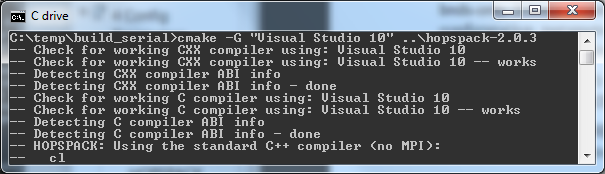
\includegraphics[width=5.5in]{winconsole_cmake_msvc.png}
\end{center}

First, make sure environment variables are configured for the Microsoft compiler.
If installed in its default location, this is accomplished (for version 10.0)
by running:
\vspace{-11pt}
\begin{tabbing}
  xxx \= \kill
  \> {\tt > c:$\backslash$Program Files$\backslash$Microsoft Visual Studio 10.0$\backslash$VC$\backslash$bin$\backslash$vcvars32.bat}
\end{tabbing}

Start at the directory where the HOPSPACK parent directory exists and
run the following commands:
\vspace{-11pt}
\begin{tabbing}
  xxx \= \kill
  \> {\tt > mkdir build\_serial} \\
  \> {\tt > cd build\_serial} \\
  \> {\tt > cmake -G "Visual Studio 10" ..$\backslash$hopspack-\HOPSVER.x-src} \\
  \> {\tt -- Check for working CXX compiler using: Visual Studio 10} \\
  \> {\tt -- ...} \\
  \> {\tt -- Build files have been written to: ...}
\end{tabbing}
\vspace{-11pt}
The execution of {\tt cmake} displays several lines of informational output,
only a few of which are shown above.
It produces a subdirectory structure similar to that of
{\sf hopspack-\HOPSVER.x-src},
and a file {\sf ALL\_BUILDS.vcxproj} with the main Visual Studio project.

Start Visual Studio and open the file {\sf ALL\_BUILDS.vcxproj}.  It contains
projects for all the libraries and executables built by HOPSPACK.
If you build {\tt ALL\_BUILDS} then Visual Studio will compile and link
everything, including the serial HOPSPACK executable, examples, and tests.
A successful build is shown in the screen shot below.

\begin{center}
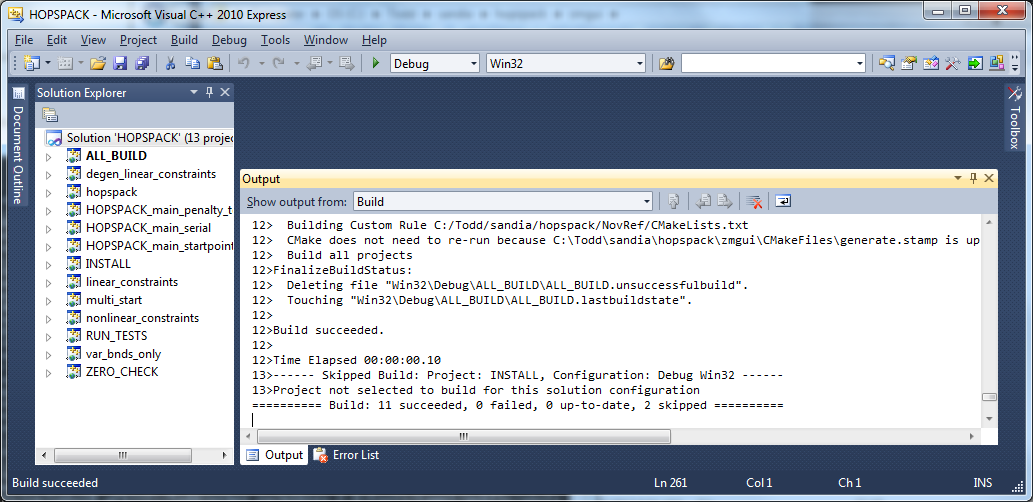
\includegraphics[width=5.0in]{winmsvc_build.png}
\end{center}

You must return to a command line console to run HOPSPACK.
The main executable should be under the {\sf src} directory:
{\sf build\_serial$\backslash$src$\backslash$src-main$\backslash$Debug$\backslash$HOPSPACK\_main\_serial.exe} in this example.  You can move the file to a
more convenient location if desired.

Now open a command line console and change to the {\sf examples} directory.
There should be a number of
subdirectories named {\sf 1-var-bnds-only, 2-linear-constraints}, etc.,
and a {\sf README.txt} file.  Each subdirectory contains HOPSPACK
configuration parameters and a small executable that evaluates optimization
objectives and constraints at a given point.
You may have to edit the parameters file in each example and tell it where
the optimization executable is located.
Run the first example:
\vspace{-11pt}
\begin{tabbing}
  xxx \= xxxxx \= \kill
  \> {\tt > cd examples$\backslash$1-bnd-vars-only} \\
  \> Edit {\sf example1\_params.txt} and change the ``Executable Name'' parameter
     to be \\
  \> \> {\tt "Executable Name" string "Debug$\backslash$var\_bnds\_only.exe"} \\
  \> {\tt > ..$\backslash$..$\backslash$src$\backslash$src-main$\backslash$Debug$\backslash$HOPSPACK\_main\_serial.exe example1\_params.txt}
\end{tabbing}
\vspace{-11pt}
As explained in the {\sf README.txt} file, this solves a simple two-dimensional
minimization problem with bound constraints.  Check the solution against
the value listed in {\sf README.txt}.
Try {\sf 2-linear-constraints} if your configuration includes an LAPACK file
for problems with linear constraints.


\bigskip
\noindent {\bf Windows using NMake (build serial HOPSPACK).}
CMake can generate a set of {\tt Makefile} files that work with the
Visual Studio command line {\tt nmake} tool.  The {\tt nmake} facility is
provided with the full Microsoft Visual Studio product or the free
Visual Studio Express Edition (available from Microsoft).

This section assumes {\it Visual C++ 2010 Express Edition} with the
version 10.0 compiler is installed.  All commands are run from
a Windows DOS-like command line console such as the one below.

\begin{center}
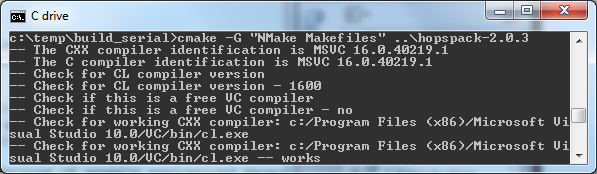
\includegraphics[width=5.5in]{winconsole_cmake.png}
\end{center}

First, make sure environment variables are configured for the Microsoft compiler.
If installed in its default location, this is accomplished (for version 10.0)
by running:
\vspace{-11pt}
\begin{tabbing}
  xxx \= \kill
  \> {\tt > c:$\backslash$Program Files$\backslash$Microsoft Visual Studio 10.0$\backslash$VC$\backslash$bin$\backslash$vcvars32.bat}
\end{tabbing}

Start at the directory where the HOPSPACK parent directory exists and
run the following commands:
\vspace{-11pt}
\begin{tabbing}
  xxx \= \kill
  \> {\tt > mkdir build\_serial} \\
  \> {\tt > cd build\_serial} \\
  \> {\tt > cmake -G "NMake Makefiles"
            ..$\backslash$hopspack-\HOPSVER.x-src} \\
  \> {\tt -- The CXX compiler identification is MSVC ...} \\
  \> {\tt -- ...} \\
  \> {\tt -- Build files have been written to: ...} \\
  \> {\tt > nmake} \\
  \> {\tt > nmake install}
\end{tabbing}
\vspace{-11pt}
The execution of {\tt cmake} displays several lines of informational output,
only a few of which are shown above.
It produces a subdirectory structure similar to that of
{\sf hopspack-\HOPSVER.x-src},
with {\tt Makefile} files that work with the chosen compiler.  Running
{\tt nmake} from the command line produces the HOPSPACK executable, test
executables, and optimization evaluators in {\sf examples}.
Running {\tt nmake install} copies appropriate files into a new subdirectory
named {\sf installed\_HOPSPACK}.

Now change to the {\sf installed\_HOPSPACK$\backslash$examples} directory.
There should be a number of
subdirectories named {\sf 1-var-bnds-only, 2-linear-constraints}, etc.,
and a {\sf README.txt} file.  Each subdirectory contains HOPSPACK
configuration parameters and a small executable that evaluates optimization
objectives and constraints at a given point.
Run the first example:
\vspace{-11pt}
\begin{tabbing}
  xxx \= \kill
  \> {\tt > cd examples$\backslash$1-bnd-vars-only} \\
  \> {\tt > ..$\backslash$..$\backslash$HOPSPACK\_main\_serial.exe example1\_params.txt}
\end{tabbing}
\vspace{-11pt}
As explained in the {\sf README.txt} file, this solves a simple two-dimensional
minimization problem with bound constraints.  Check the solution against
the value listed in {\sf README.txt}.
Try {\sf 2-linear-constraints} if your configuration includes an LAPACK file
for problems with linear constraints.


%%%%%%%%%%%%%%%%%%%%
\subsection{Build and Test an ``mt'' HOPSPACK Executable}
\label{subinstall:MT}

This section assumes you are making an ``out of source'' multithreaded build
in a separate directory from the serial build of Section~\ref{subinstall:SR}.
After building and installing at the default location,
the directory structure will look like the following (not all files are shown):
\vspace{-11pt}
\begin{tabbing}
  xxxxxxxxx \= xxx \= xxx \= xxx \= xxxxxxxxxxxxxxxxxx \= \kill
  \> {\sf hopspack-\HOPSVER.x-src}  \\
  \> \> {\sf doc}                      \> \> \> (provided)    \\
  \> \> {\sf examples}                 \> \> \> (provided)    \\
  \> \> {\sf src}                      \> \> \> (provided)    \\
  \> \> {\sf test}                     \> \> \> (provided)    \\
  \> {\sf build\_mt}                \> \> \> \> (create this and build in it)  \\
  \> \> {\sf installed\_HOPSPACK}      \> \> \> (built by CMake install)  \\
  \> \> \> {\tt HOPSPACK\_main\_threaded} \> \> (built by CMake install)  \\
  \> \> \> {\sf examples}                 \> \> (built by CMake install)  \\
  \> \> \> \> {\sf 1-var-bnds-only}          \> (built by CMake install)  \\
  \> \> \> \> {\sf ...}                      \> (built by CMake install)  \\
  \> \> \> {\sf test}                     \> \> (built by CMake install)
\end{tabbing}

The build procedure is almost identical to that of Section~\ref{subinstall:SR}.
An extra option is passed to CMake that instructs it to find
multithreading libraries and compile additional thread-based source files.
You can create separate serial and MPI versions of HOPSPACK if for some
reason multithreading libraries are not available on your machine.

All the examples in Section~\ref{subinstall:SR} begin with three instructions:
create a new directory, change to it, and run CMake.
To build the multithreaded version, similar instructions are typed
in at the command line, but with the option {\tt -Dmt=yes}:
\vspace{-11pt}
\begin{tabbing}
  xxx \= \kill
  \> {\tt > mkdir build\_mt} \\
  \> {\tt > cd build\_mt} \\
  \> {\tt > cmake ../hopspack-\HOPSVER.x-src -Dmt=yes}
\end{tabbing}

From this point, the build procedure is identical to Section~\ref{subinstall:SR}.
Note that CMake accepts any of the option values {\tt -Dmt=yes}, {\tt -Dmt=true},
or {\tt -Dmt=on}.

Assuming the build completed successfully, change to the {\sf examples}
directory.  There should be a number of subdirectories named
{\sf 1-var-bnds-only, 2-linear-constraints}, etc., and a {\sf README.txt} file.
Each subdirectory contains HOPSPACK configuration parameters and a small
executable that evaluates optimization objectives and constraints at a given
point.
Run the first example:
\vspace{-11pt}
\begin{tabbing}
  xxx \= \kill
  \> {\tt > cd examples/1-var-bnds-only} \\
  \> {\tt > ../../HOPSPACK\_main\_threaded example1\_params.txt}
\end{tabbing}
\vspace{-11pt}
As explained in the {\sf README.txt} file, this solves a simple two-dimensional
minimization problem with bound constraints.  Check the solution against
the value listed in {\sf README.txt}.
The {\tt Number Threads} parameter in the ``Mediator'' sublist
(\PGREF{param:MD-numthreads}) determines how many threads are created.
Try increasing the number of threads and observe that more ``Eval workers''
are used.

If the {\tt Display} parameter in the ``Mediator'' sublist
(\PGREF{param:MD-display}) is 3 or larger,
then a timing report for each evaluation worker will be printed after
HOPSPACK completes.  The value displayed is the cumulative wall clock time that
the Executor believes a worker is busy.  This should be nearly the same as the
time consumed by evaluations on a worker, assuming the machine has sufficient
processors to handle each worker thread.  However, if workers do not have
available processors when they are assigned work by the Executor, then the
displayed time will be longer than actual evaluation time.

Source files used in the multithreaded version are identical to those used
in the serial version except for the main routine
({\sf HOPSPACK\_main\_threaded.cpp} versus {\sf HOPSPACK\_main\_serial.cpp}),
and the executor
({\sf HOPSPACK\_ExecutorMultiThreaded.cpp} versus
{\sf HOPSPACK\_ExecutorSerial.cpp}).
In addition, the ``shared'' library includes classes that wrap native
threading functions ({\sf src/src-shared/HOPSPACK\_Thread*}).


%%%%%%%%%%%%%%%%%%%%
\subsection{Build and Test an ``mpi'' HOPSPACK Executable}
\label{subinstall:MP}

This section assumes you have read about building a serial executable in
Section~\ref{subinstall:SR}.  Differences for building with MPI are discussed
here, but refer to Section~\ref{subinstall:SR} for more details about building
with CMake.

This section assumes you are making an ``out of source'' MPI build in a separate
directory from the serial build of Section~\ref{subinstall:SR}.
After building and installing at the default location,
the directory structure will look like the following (not all files are shown):
\vspace{-11pt}
\begin{tabbing}
  xxxxxxxxx \= xxx \= xxx \= xxx \= xxxxxxxxxxxxxxxxxx \= \kill
  \> {\sf hopspack-\HOPSVER.x-src}  \\
  \> \> {\sf doc}                      \> \> \> (provided)    \\
  \> \> {\sf examples}                 \> \> \> (provided)    \\
  \> \> {\sf src}                      \> \> \> (provided)    \\
  \> \> {\sf test}                     \> \> \> (provided)    \\
  \> {\sf build\_mpi}               \> \> \> \> (create this and build in it)  \\
  \> \> {\sf installed\_HOPSPACK}      \> \> \> (built by CMake install)  \\
  \> \> \> {\tt HOPSPACK\_main\_mpi}      \> \> (built by CMake install)  \\
  \> \> \> {\sf examples}                 \> \> (built by CMake install)  \\
  \> \> \> \> {\sf 1-var-bnds-only}          \> (built by CMake install)  \\
  \> \> \> \> {\sf ...}                      \> (built by CMake install)  \\
  \> \> \> {\sf test}                     \> \> (built by CMake install)
\end{tabbing}

The build procedure is almost identical to that of Section~\ref{subinstall:SR}.
An extra option is passed to CMake that instructs it to find
MPI libraries and compile with an MPI-aware compiler.
You can create separate serial and multithreaded versions of HOPSPACK if for
some reason MPI fails to build on your machine.

All the examples in Section~\ref{subinstall:SR} begin with three instructions:
create a new directory, change to it, and run CMake.
To build the MPI version, similar instructions are typed
in at the command line, but with the option {\tt -Dmpi=yes}:
\vspace{-11pt}
\begin{tabbing}
  xxx \= \kill
  \> {\tt > mkdir build\_mpi} \\
  \> {\tt > cd build\_mpi} \\
  \> {\tt > cmake ../hopspack-\HOPSVER.x-src -Dmpi=yes}
\end{tabbing}
\vspace{-11pt}
If CMake has trouble finding your MPI-aware compiler, try specifying
it as a command line parameter; for example:
\vspace{-11pt}
\begin{tabbing}
  xxx \= \kill
  \> {\tt > cmake ../hopspack-\HOPSVER.x-src -Dmpi=yes
            -DMPI\_COMPILER=/tmp/mpich-1.2.7p1/bin/mpicxx}
\end{tabbing}
\vspace{-11pt}
If this fails, consider modifying {\sf ConfigureMPI.cmake}.  This file contains
some comments about the procedure CMake uses to find and configure MPI.

From this point, the build procedure is identical to Section~\ref{subinstall:SR}.
Note that CMake accepts any of the option values {\tt -Dmpi=yes},
{\tt -Dmpi=true}, or {\tt -Dmpi=on}.

Assuming the build completed successfully, change to the {\sf examples}
directory.  There should be a number of subdirectories named
{\sf 1-var-bnds-only, 2-linear-constraints}, etc., and a {\sf README.txt} file.
Each subdirectory contains HOPSPACK configuration parameters and a small
executable that evaluates optimization objectives and constraints at a given
point.
Run the first example:
\vspace{-11pt}
\begin{tabbing}
  xxx \= \kill
  \> {\tt > cd examples/1-var-bnds-only} \\
  \> {\tt > mpirun -np 2 ../../HOPSPACK\_main\_mpi example1\_params.txt}
\end{tabbing}
\vspace{-11pt}
As explained in the {\sf README.txt} file, this solves a simple two-dimensional
minimization problem with bound constraints.  Check the solution against
the value listed in {\sf README.txt}.
The {\tt Number Processors} parameter in the ``Mediator'' sublist
(\PGREF{param:MD-numproc}) determines how many processors are used.
Try increasing the number (along with the argument for {\tt -np})
and observe that more ``Eval workers'' are used.

If the {\tt Display} parameter in the ``Mediator'' sublist
(\PGREF{param:MD-display}) is 3 or larger,
then a timing report for each evaluation worker will be printed after
HOPSPACK completes.  The value displayed is the cumulative wall clock time that
the Executor believes a worker is busy.  Time is measured by the Executor on
the main MPI node, not the worker.  The Executor measures from the moment
an MPI message is sent to a worker to the moment an MPI reply is received.

Source files used in the MPI version are identical to those used
in the serial version except for the main routine
({\sf HOPSPACK\_main\_mpi.cpp} versus {\sf HOPSPACK\_main\_serial.cpp}),
and the executor
({\sf HOPSPACK\_ExecutorMpi.cpp} versus
{\sf HOPSPACK\_ExecutorSerial.cpp}).
In addition, the ``shared'' library includes a class that wraps MPI
functions ({\sf src/src-shared/HOPSPACK\_GenProcComm}).


%%%%%%%%%%%%%%%%%%%%
\subsection{List of Build Options for HOPSPACK}
\label{subinstall:ED}

The list below describes HOPSPACK build options available at the CMake
command line.  All options should be preceded with ``{\tt -D}''.
If the option is a Boolean flag, then the option should be followed
with ``{\tt =true}'' or ``{\tt =false}'' with no intervening spaces.

\begin{itemize}
  \item {\tt mt} $\;$
      Boolean option that instructs CMake to build a parallel HOPSPACK with
      multithreading.  See Section~\ref{subinstall:MT}.
  \item {\tt mpi} $\;$
      Boolean option that instructs CMake to build a parallel HOPSPACK for MPI.
      See Section~\ref{subinstall:MP}.
  \item {\tt lapack} $\;$
      Boolean option that instructs CMake to link with LAPACK for optimization
      problems with linear constraints.  The option is true by default.
      See Section~\ref{subinstall:LA}.
  \item {\tt LAPACK\_LIBS} $\;$
      Set the value to the (nonstandard) location of LAPACK libraries.
      See Section~\ref{subinstall:LA}.
  \item {\tt LAPACK\_ADD\_LIBS} $\;$
      Set the value to the location of additional libraries needed to
      satisfy LAPACK link dependencies.
      See Section~\ref{subinstall:LA}.
  \item {\tt HAVE\_CDDLIB} $\;$
      Boolean option that instructs CMake to include CDDLIB code for
      optimization problems with degenerate linear constraints.  The option
      is true by default.  If CDDLIB is disabled, then
      {\sf examples/3-degen-linear-constraints} will fail.
      Including CDDLIB changes the open source license status of HOPSPACK;
      see Section~\ref{subintro:licenses} for details.
  \item {\tt CMAKE\_INSTALL\_PREFIX} $\;$
      Set the value to the name of a directory where CMake should install
      final executables and examples.  The default is a directory named
      {\sf installed\_HOPSPACK} under the build directory where CMake
      is invoked.
  \item {\tt HOPSPACK\_DEBUG} $\;$
      Boolean option that instructs the native compiler to create
      a debuggable version of HOPSPACK executables.
\end{itemize}
